 \documentclass[fullscreen=true, bookmarks=false]{beamer} % , fleqn
 \usepackage[utf8]{inputenc}
 \usepackage[english,russian]{babel}
 \usepackage{xcolor}
 \usepackage{amsmath} 
 \usetheme[numbers]{PaloAlto}

\usepackage{bm}
\usepackage{graphicx}
\graphicspath{{./img/}}

\setcounter{tocdepth}{1} % подробность оглавления
\title{Краткое введение в машинное обучение}

\begin{document}

 \begin{frame}
 \transdissolve[duration=0.2]
 \titlepage
 \end{frame}

\section*{План}

\begin{frame}
\begin{quote}
При изучении наук примеры полезнее правил\\
{\em Исаак Ньютон}
\end{quote}

\begin{quote}
Нет царских путей к геометрии\\
{\em Евклид}
\end{quote}

\end{frame}

% выводим оглавление
\begin{frame}
 \transdissolve[duration=0.2]
 %\frametitle{Содержание}
 \tableofcontents[]
\end{frame}


\section{Задача оптимизации}

%%%%%%%%%%%%%%%%%%%%%%%%%%%%%%%%%%%%%%%%%%%%%%%%%%%%%%%%%%%%%%%%%%%%%%%%%%%%%%%

\begin{frame}{}
 \frametitle{Задача про домики}
Небольшая компания производит домики для кошек. Фиксированные издержки составляют 20 тыс. руб. в месяц. Переменные издержки составляют 3 тыс. руб. на каждый проданный домик. В первый месяц по цене 6 тыс. руб. за домик было продано 100 домиков. Во второй месяц была установлена цена 8 тыс. руб. за домик, и не было продано ни одного домика. В предположении, что спрос линейно зависит от цены, определите оптимальную цену и объем продаж.
\end{frame}

%%%%%%%%%%%%%%%%%%%%%%%%%%%%%%%%%%%%%%%%%%%%%%%%%%%%%%%%%%%%%%%%%%%%%%%%%%%%%%%

\begin{frame}{}
 \frametitle{Задача про домики}
 
Пусть $x$ -- количество проданных домиков, $Q$ -- прибыль компании
\begin{gather*}
\nonumber
 c(x) = 20 + 3x\\
\nonumber
 x = 50(8-p)\\
\nonumber
 p(x) = 8-0.02x\\
\nonumber
 Q(x) = p(x)x - c(x)\\
\nonumber
 Q(x) \rightarrow max
\end{gather*}

\end{frame}

%%%%%%%%%%%%%%%%%%%%%%%%%%%%%%%%%%%%%%%%%%%%%%%%%%%%%%%%%%%%%%%%%%%%%%%%%%%%%%%

\begin{frame}{}
\frametitle{Производная и скорость}
\begin{figure}[]
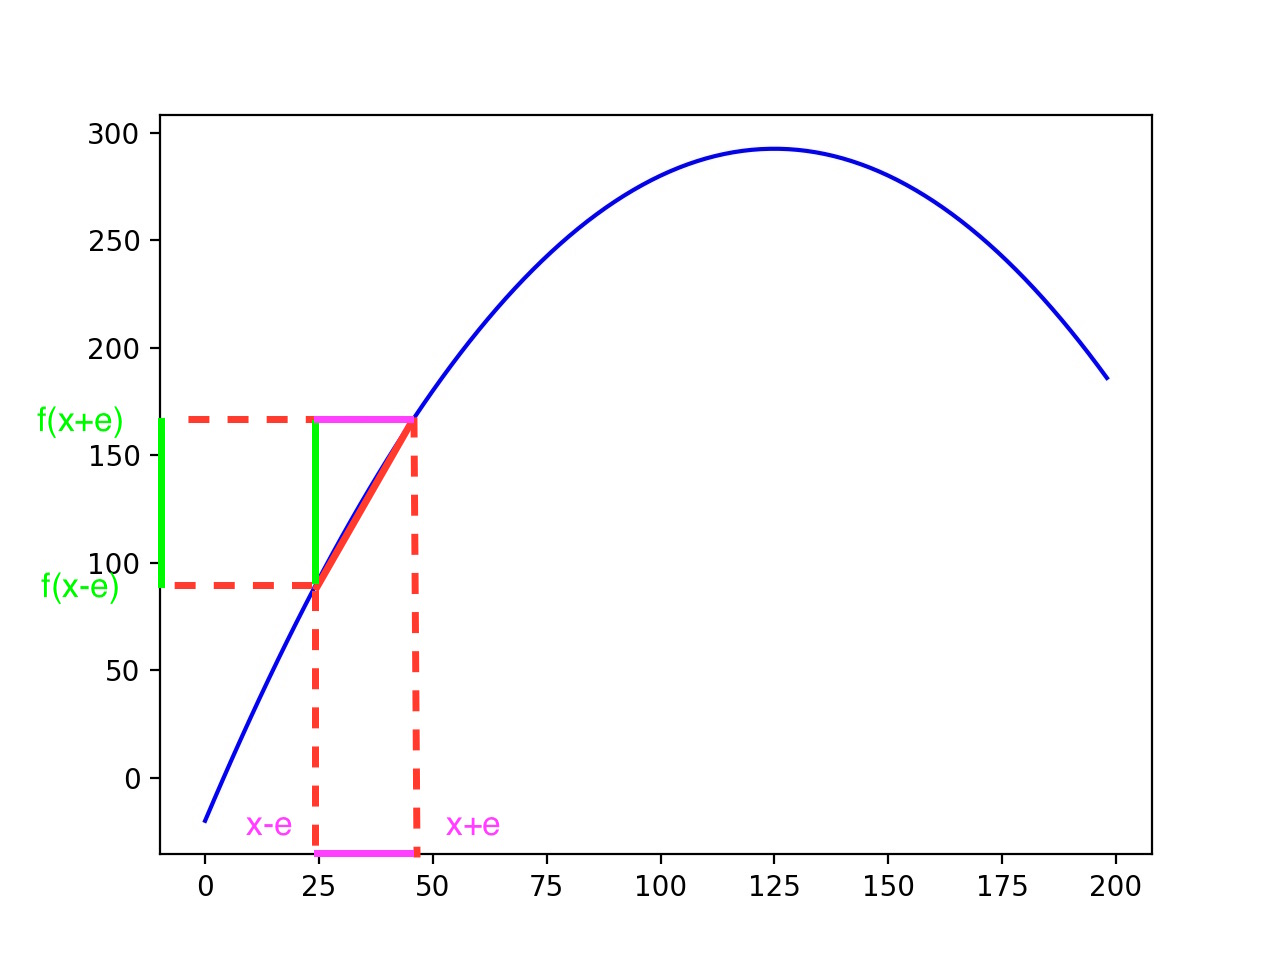
\includegraphics[scale=0.22]{der1} 
\end{figure}
\end{frame}

%%%%%%%%%%%%%%%%%%%%%%%%%%%%%%%%%%%%%%%%%%%%%%%%%%%%%%%%%%%%%%%%%%%%%%%%%%%%%%%

\begin{frame}{}
\frametitle{Производная и скорость}
\begin{figure}[]
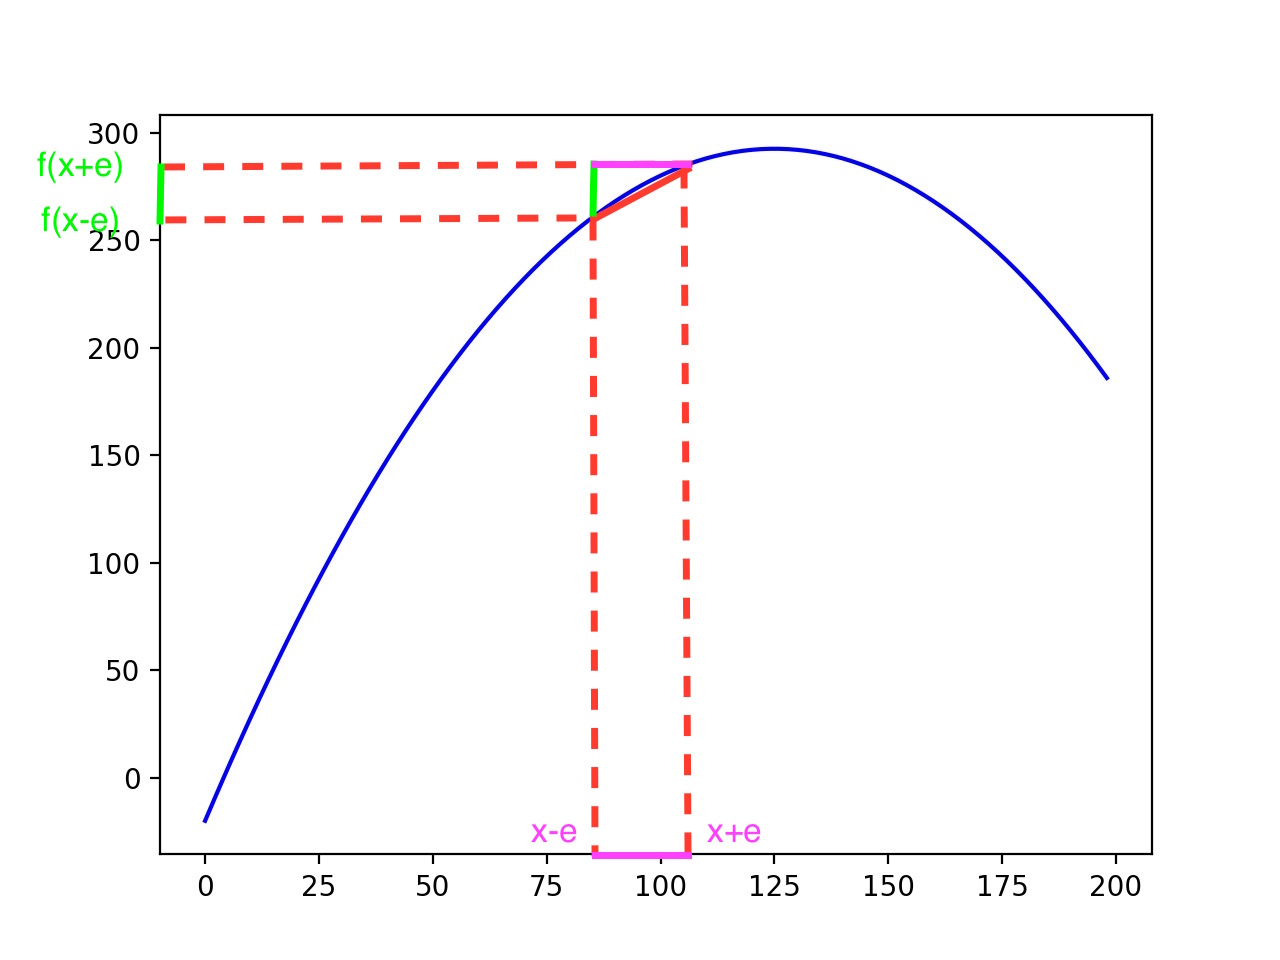
\includegraphics[scale=0.22]{der2} 
\end{figure}
\end{frame}

%%%%%%%%%%%%%%%%%%%%%%%%%%%%%%%%%%%%%%%%%%%%%%%%%%%%%%%%%%%%%%%%%%%%%%%%%%%%%%%

\begin{frame}{}
 \frametitle{Градиентный спуск}
$L(x)$ -- функция потерь (Loss function) 
\begin{gather*}
\nonumber
L(x) \rightarrow min\\
\nonumber\\
\nonumber
\text{update step: } x = x - \alpha \nabla L(x)\\
\nonumber\\
\nonumber
\nabla L(x) = \frac{L(x+\varepsilon) - L(x - \varepsilon)}{2\varepsilon}
\end{gather*}

\end{frame}

%%%%%%%%%%%%%%%%%%%%%%%%%%%%%%%%%%%%%%%%%%%%%%%%%%%%%%%%%%%%%%%%%%%%%%%%%%%%%%%

\begin{frame}{}
 \frametitle{Минимизация функции двух переменных}
$L(x_1, x_2)$ -- функция потерь 
\begin{gather*}
\nonumber
L(x_1, x_2) \rightarrow min\\
\nonumber\\
\nonumber
x_1 = x_1 - \alpha \nabla_1 L(x_1, x_2)\\
\nonumber
x_2 = x_2 - \alpha \nabla_2 L(x_1, x_2)\\
\nonumber\\
\nonumber
\nabla_1 L(x_1, x_2) = \frac{L(x_1+\varepsilon, x_2) - L(x_1 - \varepsilon, x_2)}{2\varepsilon}\\
\nonumber
\nabla_2 L(x_1, x_2) = \frac{L(x_1, x_2+\varepsilon) - L(x_1 , x_2 - \varepsilon)}{2\varepsilon}
\end{gather*}

\end{frame}

%%%%%%%%%%%%%%%%%%%%%%%%%%%%%%%%%%%%%%%%%%%%%%%%%%%%%%%%%%%%%%%%%%%%%%%%%%%%%%%

\begin{frame}{}
 \frametitle{Минимизация функции многих переменных}
\begin{gather*}
\nonumber
L(\bm{x}) \rightarrow min\\
\nonumber
\text{update step: } \bm{x} = \bm{x} - \alpha \nabla L(\bm{x})\\
\nonumber
\nonumber\\
\nonumber
\nabla_i L(\bm{x}) = \frac{L(\bm{x}_+) - L(\bm{x}_-)}{2\varepsilon}\\
\nonumber
\bm{x}_+ = [x_1, x_2, \ldots, x_i+\varepsilon, \ldots, x_n]\\
\bm{x}_- = [x_1, x_2, \ldots, x_i-\varepsilon, \ldots, x_n]
\end{gather*}

\end{frame}

%%%%%%%%%%%%%%%%%%%%%%%%%%%%%%%%%%%%%%%%%%%%%%%%%%%%%%%%%%%%%%%%%%%%%%%%%%%%%%%

\begin{frame}{}
 \frametitle{Суммы и вектора}

Знак суммы
\begin{gather*}
\nonumber
\sum_{i=1}^n a_i = a_1 + a_2 + a_3 + \ldots + a_n\\
\nonumber \\
\nonumber
\sum_i a_i = a_1 + a_2 + a_3 + \ldots + a_n\\
\end{gather*}

Вектор -- набор пронумерованных чисел (список чисел). $\bm{x} = [x_1, x_2]$ -- двумерный вектор (список из двух чисел).


Пример 1: Дан трехмерный вектор $\bm{w} = [2.3, 3.1, 7.0]$. Рассчитать $\sum_i w_i$


Пример 2: $\bm{f} = [0.0, 1.0, 0.0]$. Рассчитать $\sum_i w_i f_i$

\end{frame}

%%%%%%%%%%%%%%%%%%%%%%%%%%%%%%%%%%%%%%%%%%%%%%%%%%%%%%%%%%%%%%%%%%%%%%%%%%%%%%%

\section{Задача классификации}

%%%%%%%%%%%%%%%%%%%%%%%%%%%%%%%%%%%%%%%%%%%%%%%%%%%%%%%%%%%%%%%%%%%%%%%%%%%%%%%

\begin{frame}{}
 \frametitle{Классификация}

$\bm{f}_k$ -- вектора признаков (features) объектов (samples), $y_k$ -- номера классов объектов, $\bm{w}$ -- параметры модели. 

 Функция потерь:

\begin{gather*}
\nonumber
L(\bm{w}) = \sum_k L_k(\bm{w}) \rightarrow min\\
\end{gather*}

Функция потерь на k-м объекте:

 \begin{gather*}
 \nonumber
 L_k(\bm{w}) = |g(\bm{w}, \bm{f}_k) - y_k|\\
 \end{gather*}

 $y = g(\bm{w}, \bm{f})$ -- классифицирующая функция.

\end{frame}

%%%%%%%%%%%%%%%%%%%%%%%%%%%%%%%%%%%%%%%%%%%%%%%%%%%%%%%%%%%%%%%%%%%%%%%%%%%%%%%

\begin{frame}{}
 \frametitle{Стохастический градиентный спуск}
 
 Функция потерь:
 \begin{gather*}
 \nonumber
 L(\bm{w}) = \sum_k L_k(\bm{w}) \rightarrow min\\
 \end{gather*}

Будем обновлять параметры модели отдельно для каждого объекта (примера), а не для всей суммы сразу

\begin{gather*}
\nonumber
 \bm{w} = \bm{w} - \alpha \nabla L_k(\bm{w})\\
\end{gather*}

\end{frame}

%%%%%%%%%%%%%%%%%%%%%%%%%%%%%%%%%%%%%%%%%%%%%%%%%%%%%%%%%%%%%%%%%%%%%%%%%%%%%%%

\begin{frame}{}
 \frametitle{Линейная функция}
 $\bm{w}$, $b$ -- коэффициенты линейной функции
\begin{gather*}
\nonumber
l(\bm{x}) = b + \sum_i w_i x_i
\end{gather*}

Двумерный случай
\begin{gather*}
\nonumber
l(\bm{x}) = b + \sum_{i=0}^1 w_i x_i= b + w_0 x_0 + w_1 x_1
\end{gather*}

\end{frame}

%%%%%%%%%%%%%%%%%%%%%%%%%%%%%%%%%%%%%%%%%%%%%%%%%%%%%%%%%%%%%%%%%%%%%%%%%%%%%%%

\begin{frame}{}
 \frametitle{Сигмоид}
\begin{gather*}
\nonumber
\sigma(x) = \frac{e^x}{e^x + 1}
\end{gather*}
\begin{figure}[]
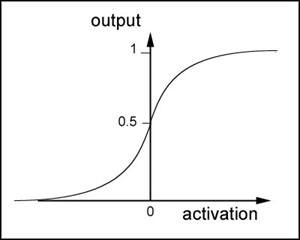
\includegraphics[scale=0.5]{sigmoid} 
%\label{fig:HolesExperiment1}
\end{figure}

\end{frame}

%%%%%%%%%%%%%%%%%%%%%%%%%%%%%%%%%%%%%%%%%%%%%%%%%%%%%%%%%%%%%%%%%%%%%%%%%%%%%%%

\begin{frame}{}
 \frametitle{Персептрон}
\begin{gather*}
\nonumber
g(\bm{x}) = \sigma(b + \sum_i w_i x_i)
\end{gather*}

\begin{figure}[]
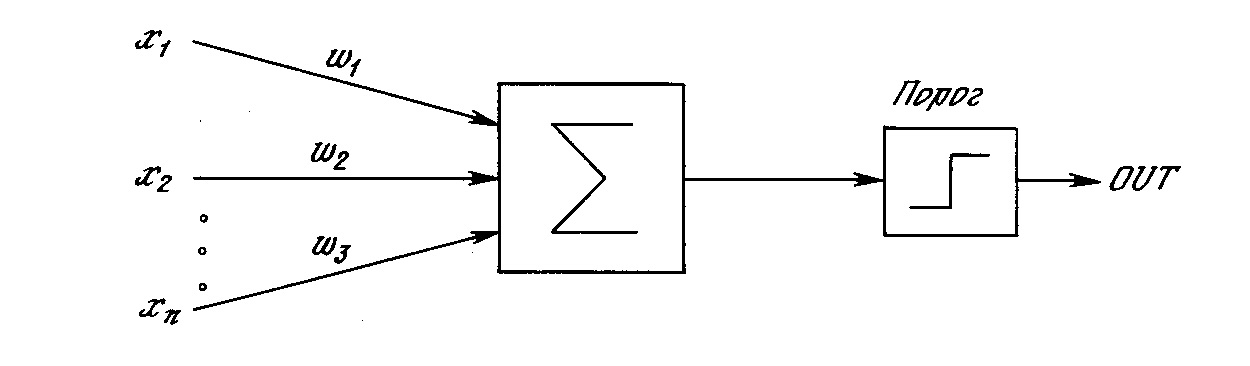
\includegraphics[scale=0.2]{perceptron} 
\end{figure}

\end{frame}

%%%%%%%%%%%%%%%%%%%%%%%%%%%%%%%%%%%%%%%%%%%%%%%%%%%%%%%%%%%%%%%%%%%%%%%%%%%%%%%

\begin{frame}{}
 \frametitle{Персептрон}
\begin{gather*}
\nonumber
g(\bm{x}) = \sigma(b + \sum_i w_i x_i)
\end{gather*}

Уравнение
\begin{gather*}
\nonumber
g(\bm{x}) = 0.5\\
\nonumber
b + \sum_i w_i x_i = 0\\
\end{gather*}
задает поверхность, разделяющую классы.
\end{frame}


%%%%%%%%%%%%%%%%%%%%%%%%%%%%%%%%%%%%%%%%%%%%%%%%%%%%%%%%%%%%%%%%%%%%%%%%%%%%%%%

\section{Состояние современной науки}

%%%%%%%%%%%%%%%%%%%%%%%%%%%%%%%%%%%%%%%%%%%%%%%%%%%%%%%%%%%%%%%%%%%%%%%%%%%%%%%

\begin{frame}{}
\frametitle{Как было раньше}
\begin{figure}[]
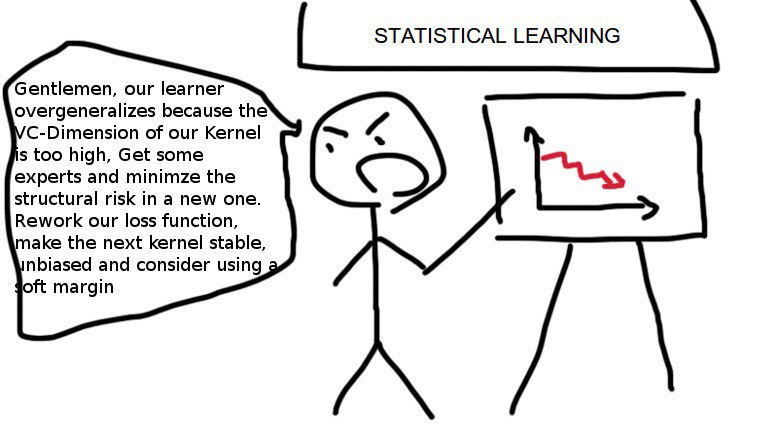
\includegraphics[scale=0.4]{past} 
\end{figure}

\footnotetext{https://vk.com/weirdkerneltricks}

\end{frame}

%%%%%%%%%%%%%%%%%%%%%%%%%%%%%%%%%%%%%%%%%%%%%%%%%%%%%%%%%%%%%%%%%%%%%%%%%%%%%%%

\begin{frame}{}
\frametitle{Как теперь}
\begin{figure}[]
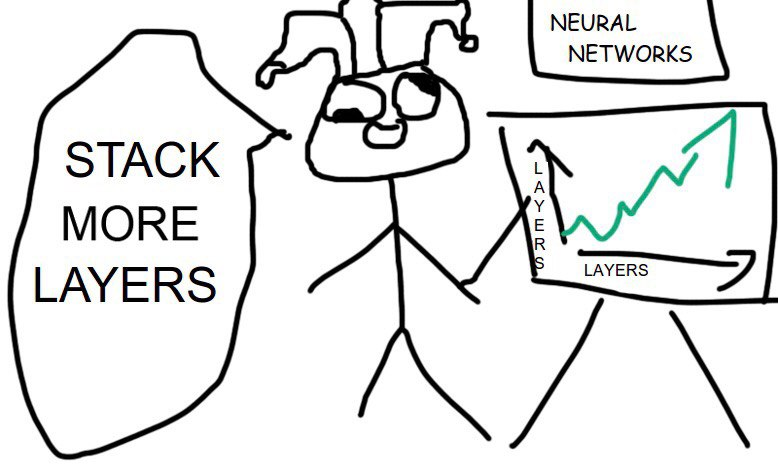
\includegraphics[scale=0.35]{future} 
\end{figure}

\footnotetext{https://vk.com/weirdkerneltricks}

\end{frame}

%%%%%%%%%%%%%%%%%%%%%%%%%%%%%%%%%%%%%%%%%%%%%%%%%%%%%%%%%%%%%%%%%%%%%%%%%%%%%%%

%%%%%%%%%%%%%%%%%%%%%%%%%%%%%%%%%%%%%%%%%%%%%%%%%%%%%%%%%%%%%%%%%%%%%%%%%%%%%%%

\section{Что делать дальше?}

%%%%%%%%%%%%%%%%%%%%%%%%%%%%%%%%%%%%%%%%%%%%%%%%%%%%%%%%%%%%%%%%%%%%%%%%%%%%%%%

\begin{frame}
\begin{quote}
Математика — это язык, на котором написана книга природы.\\
{\em Галилео Галилей}
\end{quote}

\end{frame}

%%%%%%%%%%%%%%%%%%%%%%%%%%%%%%%%%%%%%%%%%%%%%%%%%%%%%%%%%%%%%%%%%%%%%%%%%%%%%%%

\end{document}